\section{アンケート結果}
\ref{調査項目}の表\ref{table:anque}で述べたそれぞれのアンケート項目の結果とその評価について述べる.

\subsection{結果}
初めにゲームが与える子どもの発育や成長への影響の全体的な印象についての質問をサイトを見る前と見た後の項目に分け,1から5の5段階評価で行った.


\begin{figure}[H]
 \begin{center}
  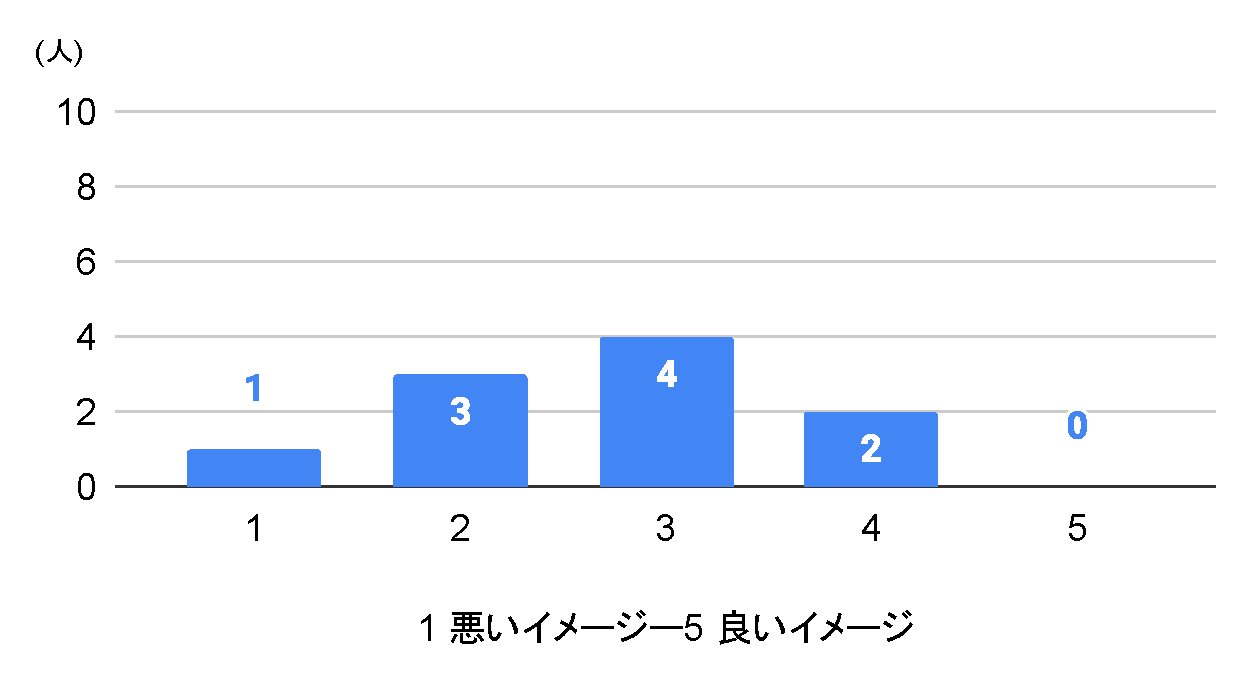
\includegraphics[keepaspectratio, scale=0.6]{PDF/印象前.pdf}
 \end{center}
 \caption{サイトを見る前はゲームが子どもの発育・成長へ与える影響に対して大まかにどのようなイメージを持っていたか}
 \label{fig:見る前印象}
\end{figure}

\begin{figure}[H]
 \begin{center}
  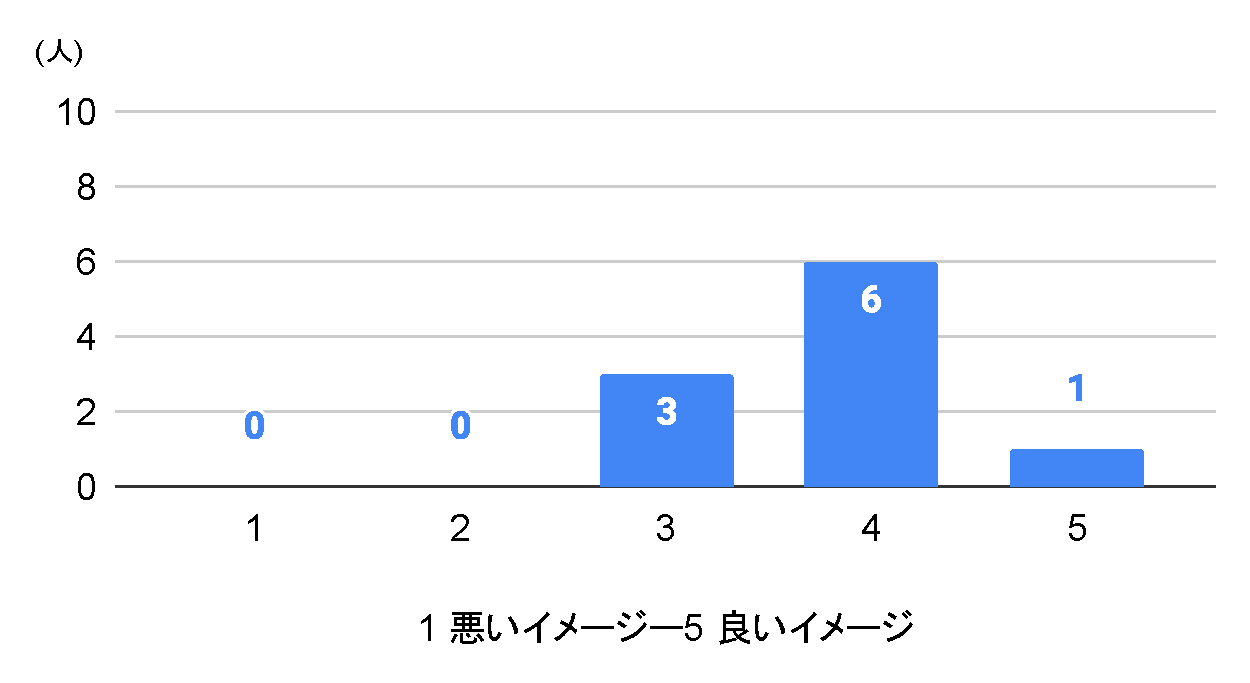
\includegraphics[keepaspectratio, scale=0.6]{PDF/印象後.pdf}
 \end{center}
 \caption{サイトを見た後はゲームが子どもの発育・成長へ与える影響に対して大まかにどのようなイメージを持ったか}
 \label{fig:見た後印象}
\end{figure}

図\ref{fig:見る前印象}に示すように対象者にWebサイトを見てもらう前の印象はやや良いイメージである4が2人と少なくどちらでもないから悪いイメージを持つ人が多くみられた.
しかし図\ref{fig:見た後印象}に示すようにWebサイトを見た後の全体的な印象はどちらでもないが3票あったもののやや良いイメージと良いイメージがあると答えた人が7人に増加した.

2番目にゲームが勉強面に与える影響について1の悪い影響があると思うから5の良い影響があると思うの5段階評価で行った.
図\ref{fig:勉強前}に示すようにWebサイトを見る前は2のやや悪い影響があると思うを選択した人は8人と多かった.
図\ref{fig:勉強後}に示すように見た後はどちらとも言えないを選択した人が多くを占めたがやや良い影響があると思う・良い影響があると思うを選択した人が増加した.
またまだやや悪い影響があると思うを選択した人1人いた.

\begin{figure}[H]
 \begin{center}
  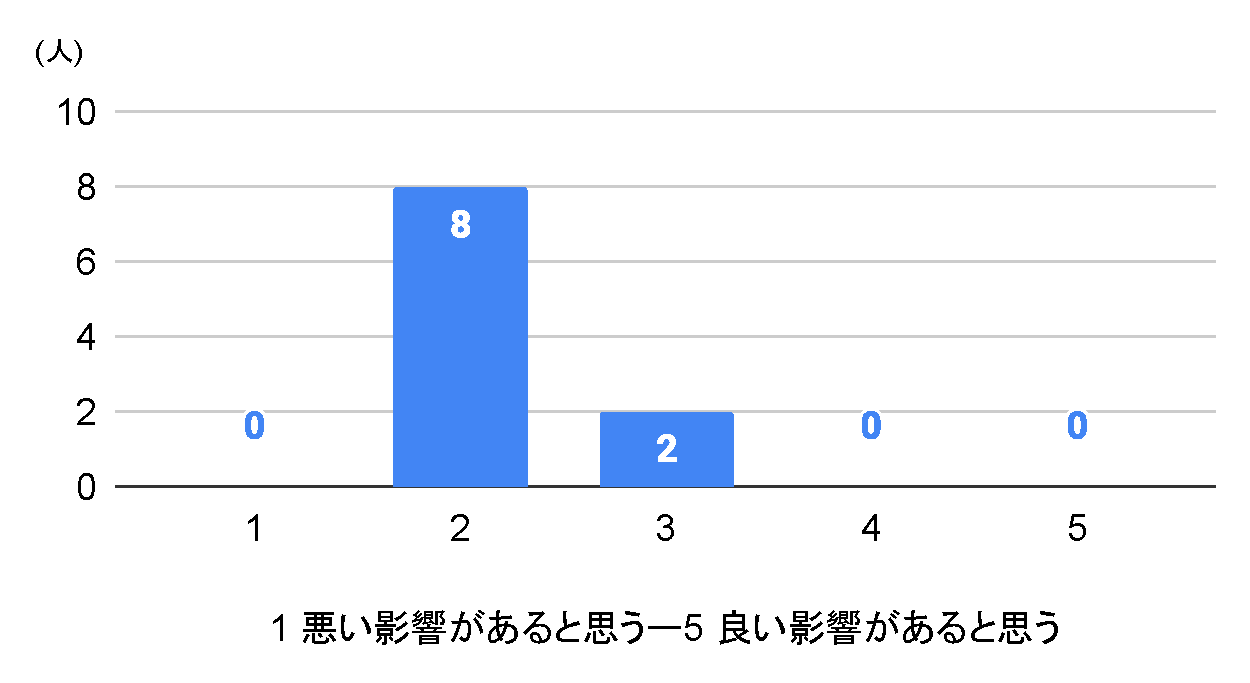
\includegraphics[keepaspectratio, scale=0.6]{PDF/勉強前.pdf}
 \end{center}
 \caption{ゲームが勉強面に与える影響についてどのように考えていたか}
 \label{fig:勉強前}
\end{figure}

\begin{figure}[H]
 \begin{center}
  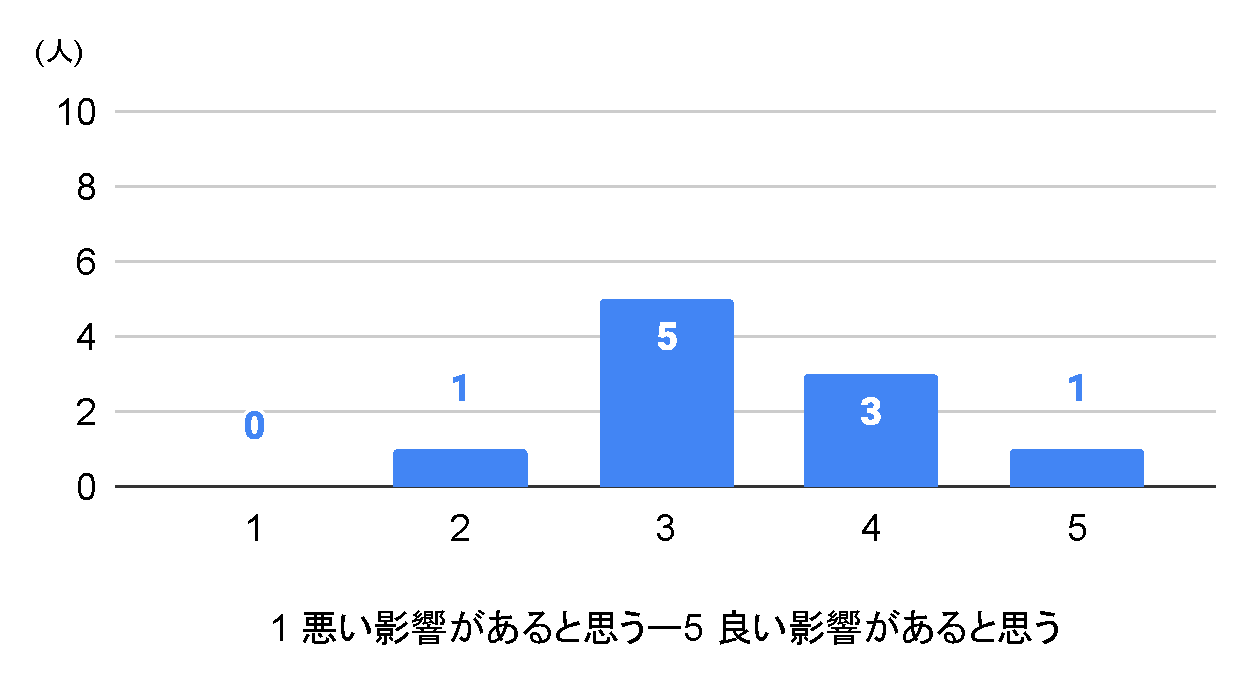
\includegraphics[keepaspectratio, scale=0.6]{PDF/勉強後.pdf}
 \end{center}
 \caption{ゲームが勉強面に与える影響についてどのように考えたか}
 \label{fig:勉強後}
\end{figure}

3番目にゲームが友人関係・コミュニケーションに与える影響について5段階評価で行った.
図\ref{fig:コミュ前}に示すようにWebサイトを見る前は悪い影響があると思う人が少なく,やや良い影響があると思うを選択する人が多かった.
図\ref{fig:コミュ後}に示すように見た後については悪い影響があると思うを選択した人は0人になりやや良い影響があると思うを選択した人が7人で多くを占めた.

\begin{figure}[H]
 \begin{center}
  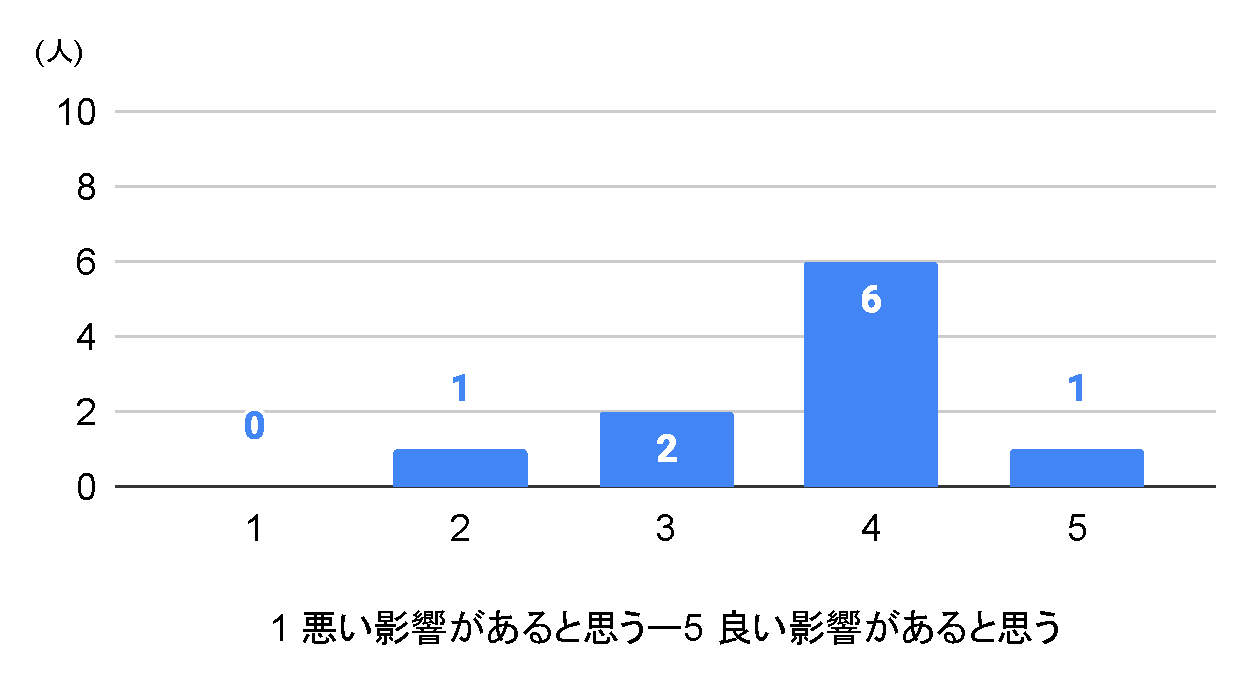
\includegraphics[keepaspectratio, scale=0.6]{PDF/コミュ前.pdf}
 \end{center}
 \caption{ゲームが友人関係・コミュニケーションに与える影響についてどのように考えていたか}
 \label{fig:コミュ前}
\end{figure}

\begin{figure}[H]
 \begin{center}
  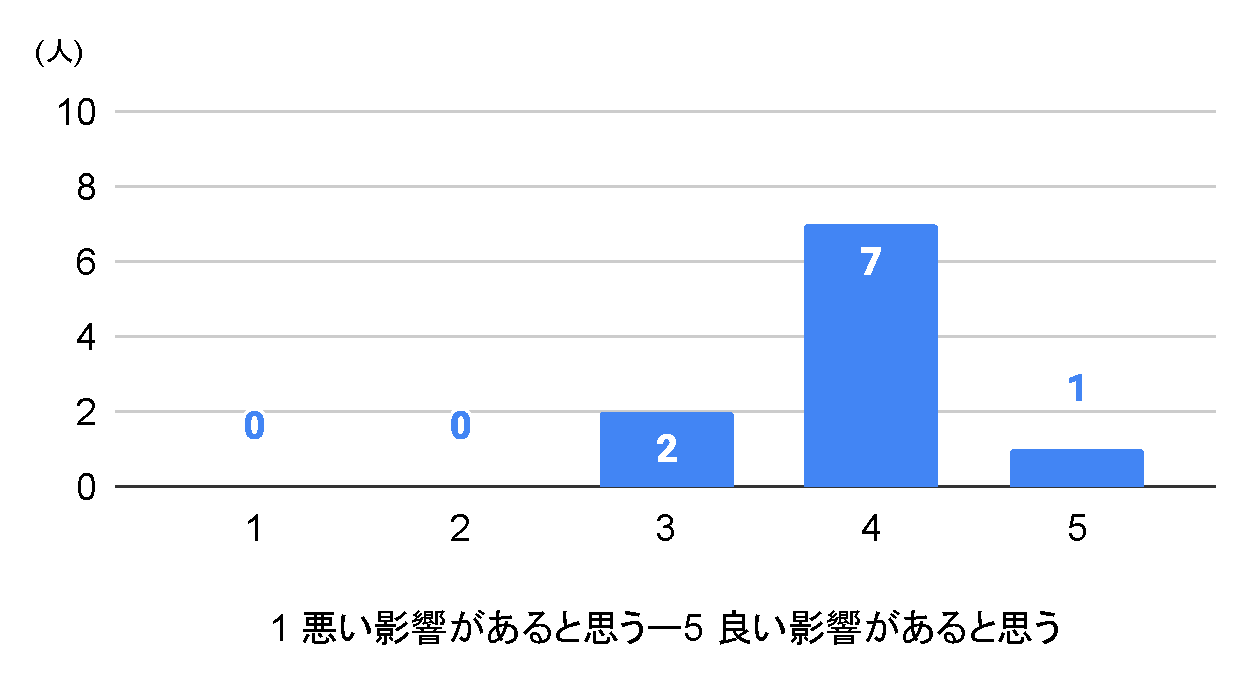
\includegraphics[keepaspectratio, scale=0.6]{PDF/コミュ後.pdf}
 \end{center}
 \caption{ゲームが友人関係・コミュニケーションに与える影響についてどのように考えたか}
 \label{fig:コミュ後}
\end{figure}

4番目にゲームが感性に与える影響について5段階評価で行った.
図\ref{fig:感性前}に示すようにWebサイトを見る前はやや良い影響があると思う傾向があったが,やや悪い影響があると思うを選択した人が少なからずいた.
一方で図\ref{fig:感性後}に示すように見た後に関しては悪い影響があると思うを選択した人が0人でやや良い影響があると思うを選択した人が6人と思うと良い影響があると思うを選択した人が3人で大半を占めた.

\begin{figure}[H]
 \begin{center}
  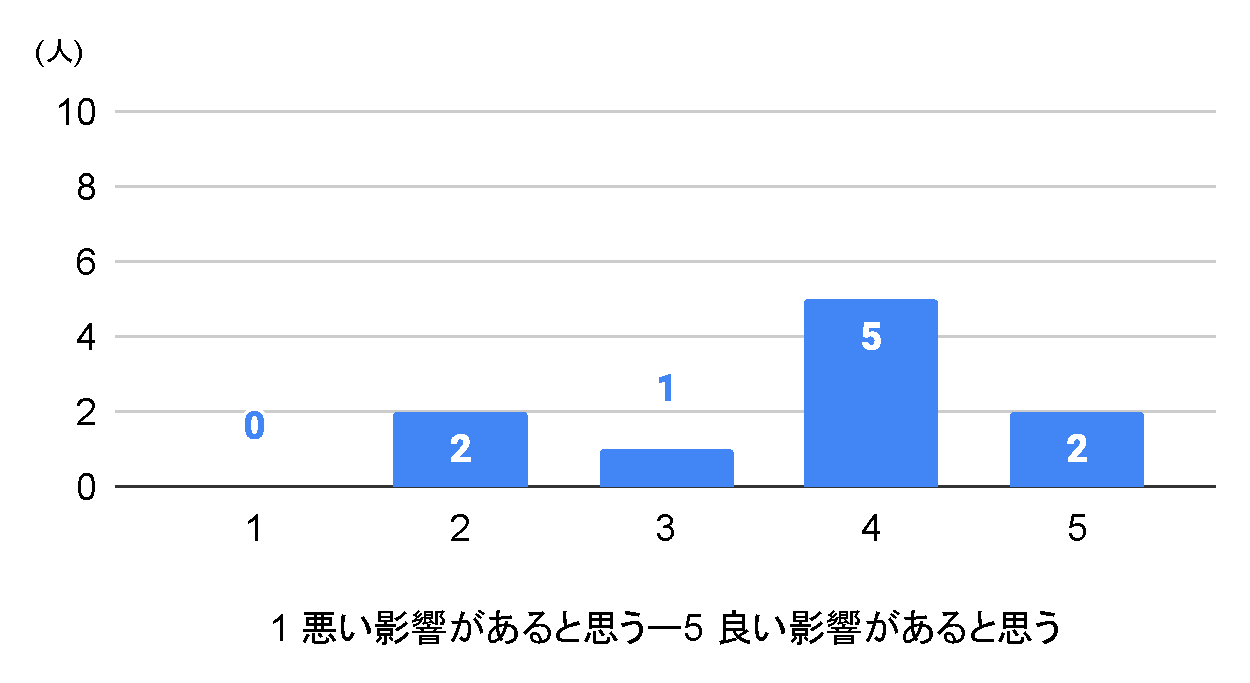
\includegraphics[keepaspectratio, scale=0.6]{PDF/感性前.pdf}
 \end{center}
 \caption{ゲームが感性に与える影響についてどのように考えていたか}
 \label{fig:感性前}
\end{figure}

\begin{figure}[H]
 \begin{center}
  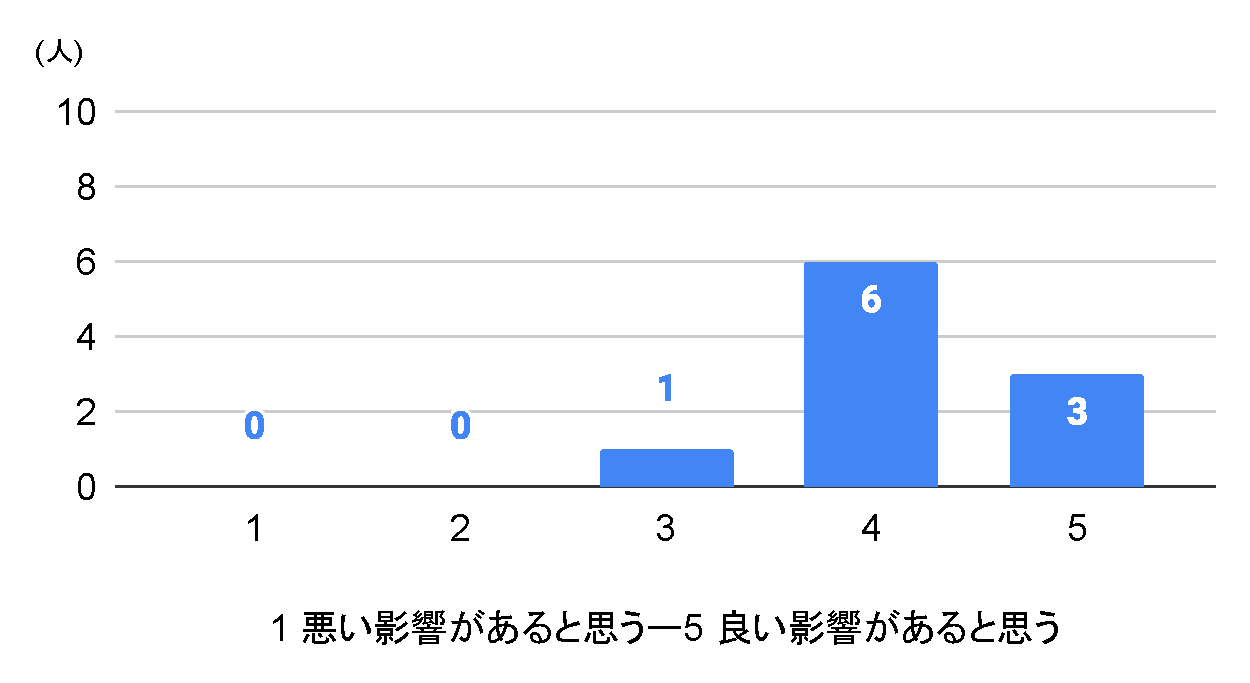
\includegraphics[keepaspectratio, scale=0.6]{PDF/感性後.pdf}
 \end{center}
 \caption{ゲームが感性に与える影響についてどのように考えたか}
 \label{fig:感性後}
\end{figure}

5番目にゲームが知識や教養面に与える影響について5段階評価で行った.
図\ref{fig:知識前}と図\ref{fig:知識後}に示すようにWebサイトを見る前と後でほとんど変わらずやや良い影響があると思うを選択した人が7人と8人で大半を占め,悪い影響がある・やや悪い影響があると思うを選択した人と思う人は0人だった.

\begin{figure}[H]
 \begin{center}
  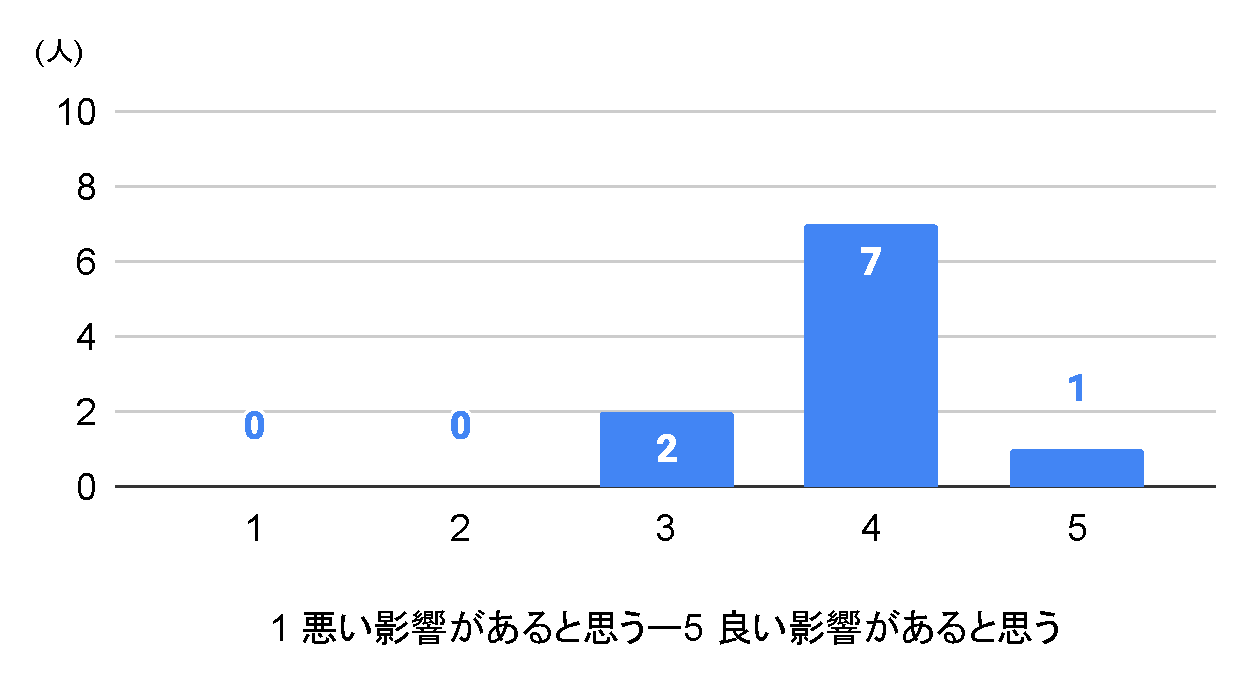
\includegraphics[keepaspectratio, scale=0.6]{PDF/知識前.pdf}
 \end{center}
 \caption{ゲームが知識・教養に与える影響についてどのように考えていたか}
 \label{fig:知識前}
\end{figure}

\begin{figure}[H]
 \begin{center}
  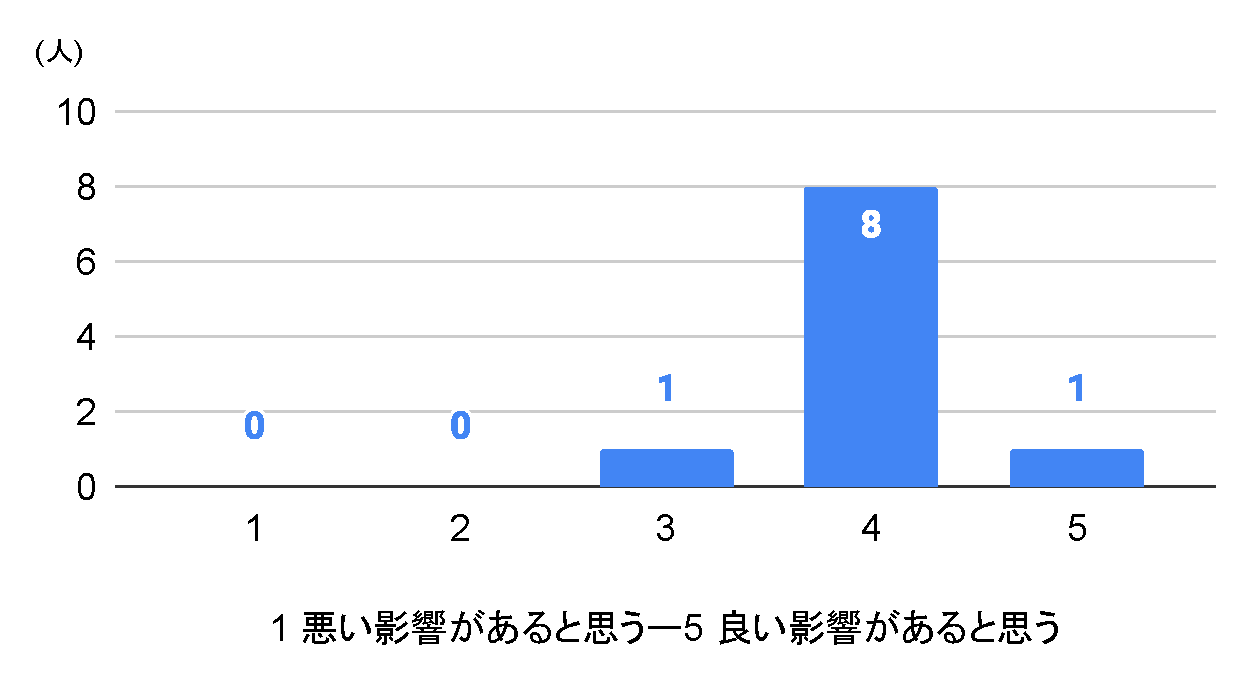
\includegraphics[keepaspectratio, scale=0.6]{PDF/知識後.pdf}
 \end{center}
 \caption{ゲームが知識・教養に与える影響についてどのように考えたか}
 \label{fig:知識後}
\end{figure}

6番目にゲームが時間管理面に与える影響について5段階評価で行った.
図\ref{fig:時間前}に示すようにWebサイトを見る前は悪い影響があると思うを選択した人が3人とやや悪い影響があると思うを選択した人が5人で多く,良い影響があると思うを選択した人は少なかった.
図\ref{fig:時間後}に示すように見た後については悪い影響があると思うを選択した人は0人だったかやや悪い影響があると思うを選択した人が6人,どちらともいえないを選択した人が3人,やや良い影響があると思うを選択した人が1人で変化は少なかった.

\begin{figure}[H]
 \begin{center}
  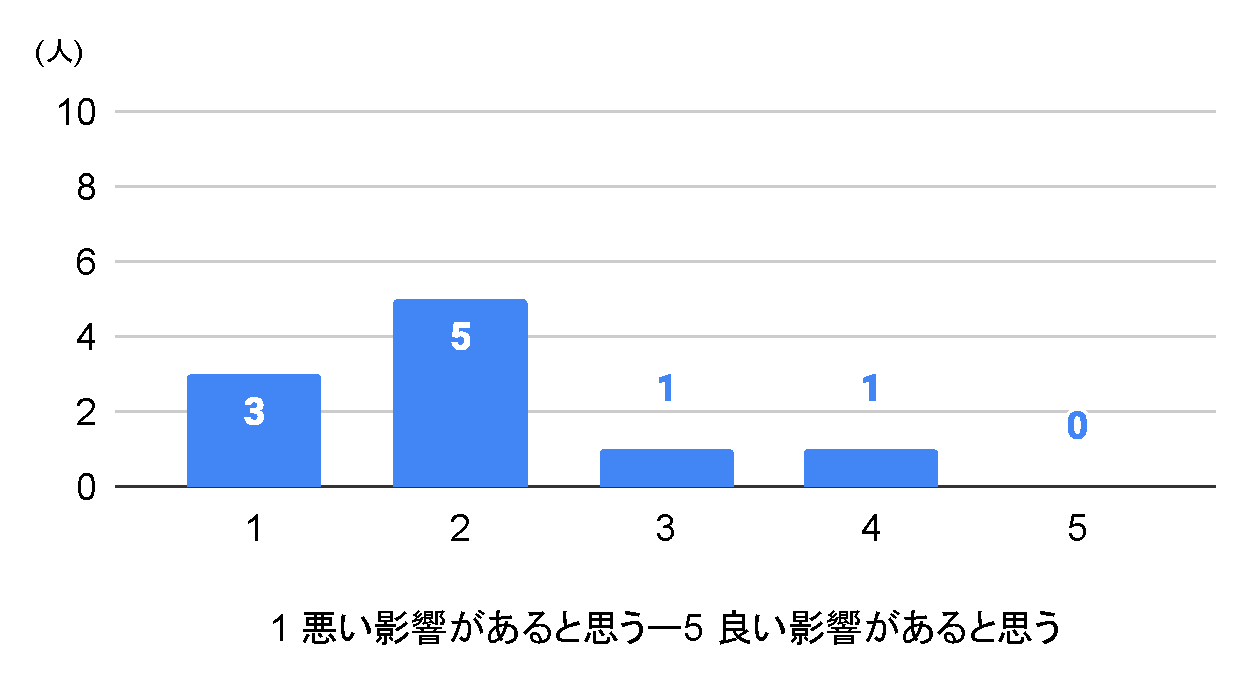
\includegraphics[keepaspectratio, scale=0.6]{PDF/時間前.pdf}
 \end{center}
 \caption{ゲームが時間管理に与える影響についてどのように考えていたか}
 \label{fig:時間前}
\end{figure}

\begin{figure}[H]
 \begin{center}
  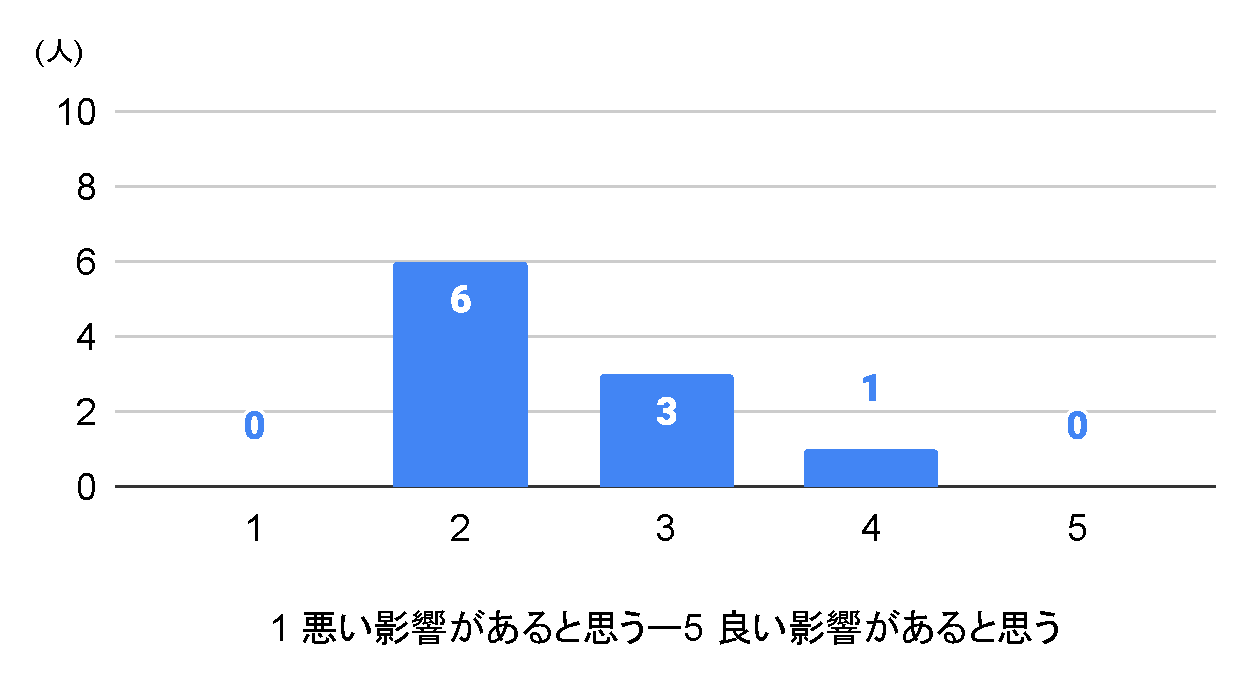
\includegraphics[keepaspectratio, scale=0.6]{PDF/時間後.pdf}
 \end{center}
 \caption{ゲームが時間管理に与える影響についてどのように考えたか}
 \label{fig:時間後}
\end{figure}

7番目にゲームが健康面に与える影響について5段階評価で行った.
図\ref{fig:健康前}に示すようにWebサイトを見る前は悪い影響があると思うを選択した人が1人,やや悪い影響があると思うを選択した人が9人で良い影響があると考える人は0人だった.
図\ref{fig:健康後}に示すように見た後については悪い影響があると考える人は2人と減りどちらとも言えないが5人,やや良い影響があると思うを選択した人が3人と少し好転した.

\begin{figure}[H]
 \begin{center}
  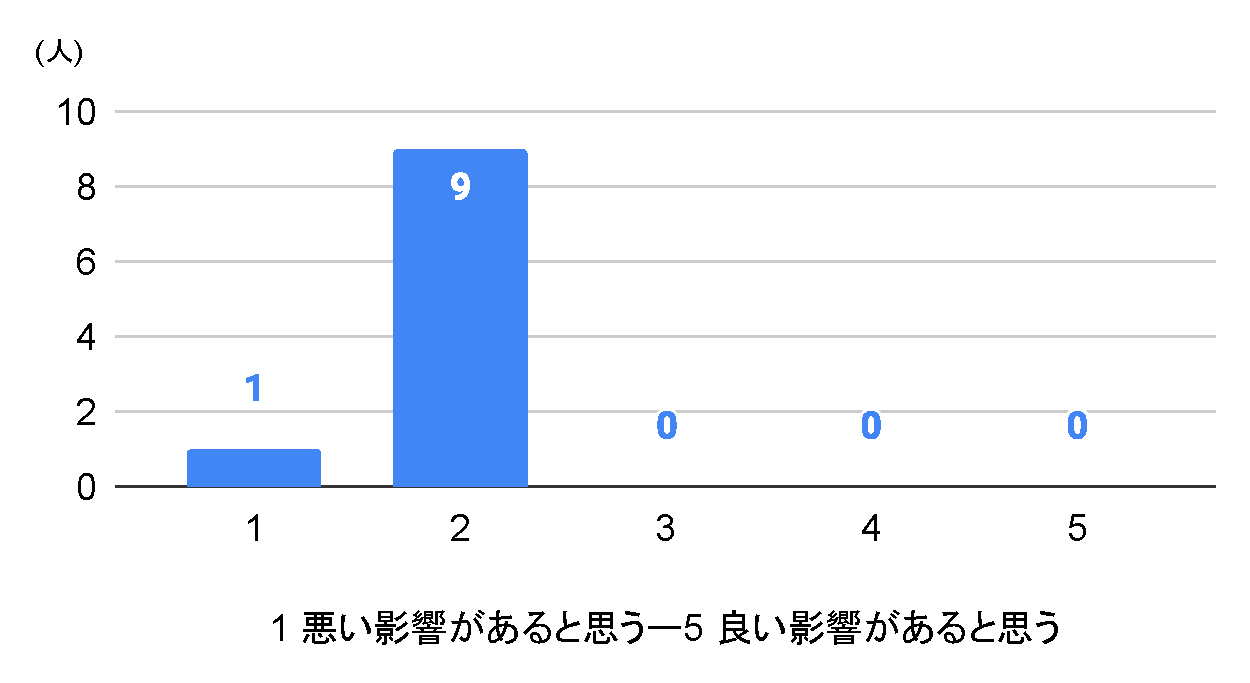
\includegraphics[keepaspectratio, scale=0.6]{PDF/健康前.pdf}
 \end{center}
 \caption{ゲームが健康面に与える影響についてどのように考えていたか}
 \label{fig:健康前}
\end{figure}

\begin{figure}[H]
 \begin{center}
  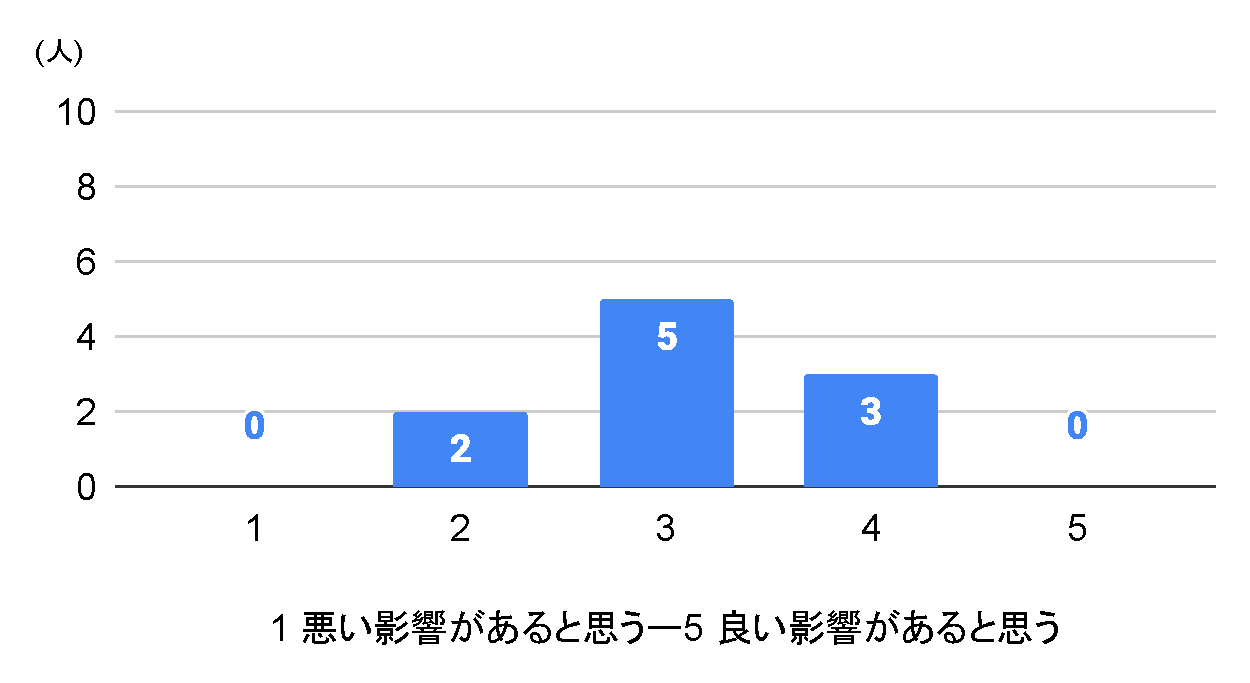
\includegraphics[keepaspectratio, scale=0.6]{PDF/健康後.pdf}
 \end{center}
 \caption{ゲームが健康面に与える影響についてどのように考えたか}
 \label{fig:健康後}
\end{figure}

8番目に読書や映画鑑賞,スポーツ,友達と遊ぶといった他の趣味や活動に比べゲームをプレイすることの利点について,デメリットが多い・それも同じくらい・メリットが多いの3選択式で行った.
図\ref{fig:比較前}に示すようにWebサイトを見る前はどれも同じくらいを選択した人が6人でデメリットが多いを選択した人が4人となりメリットが多いと考える人は0人だった.
図\ref{fig:比較後}に示すように見た後についてはどれも同じくらいを選択した人が7人に,メリットが多いを選択した人が1人に増えたが,デメリットが多いと考える人もまだいた.

\begin{figure}[H]
 \begin{center}
  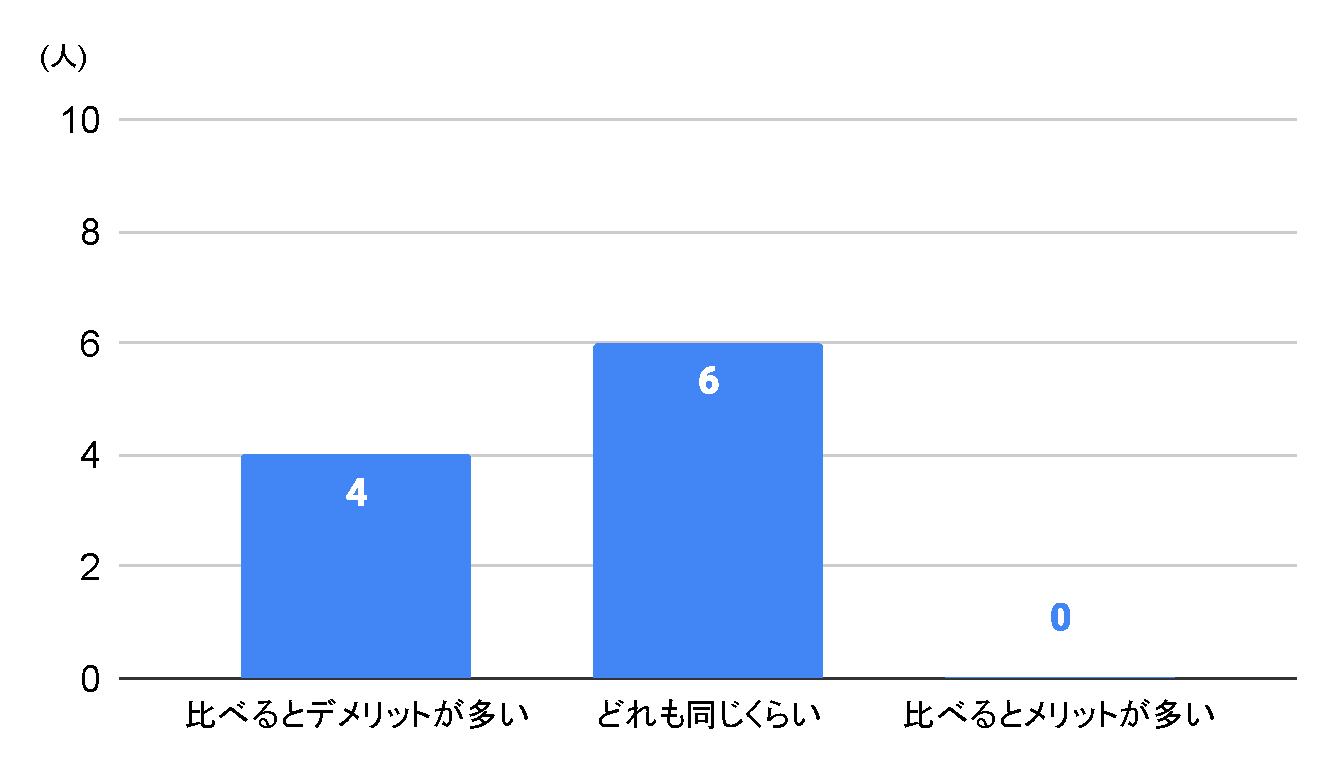
\includegraphics[keepaspectratio, scale=0.5]{PDF/比較前.pdf}
 \end{center}
 \caption{読書や映画鑑賞,スポーツ,友達と遊ぶことなど比べ,ゲームをプレイすることは利点があると思っていたか}
 \label{fig:比較前}
\end{figure}

\begin{figure}[H]
 \begin{center}
  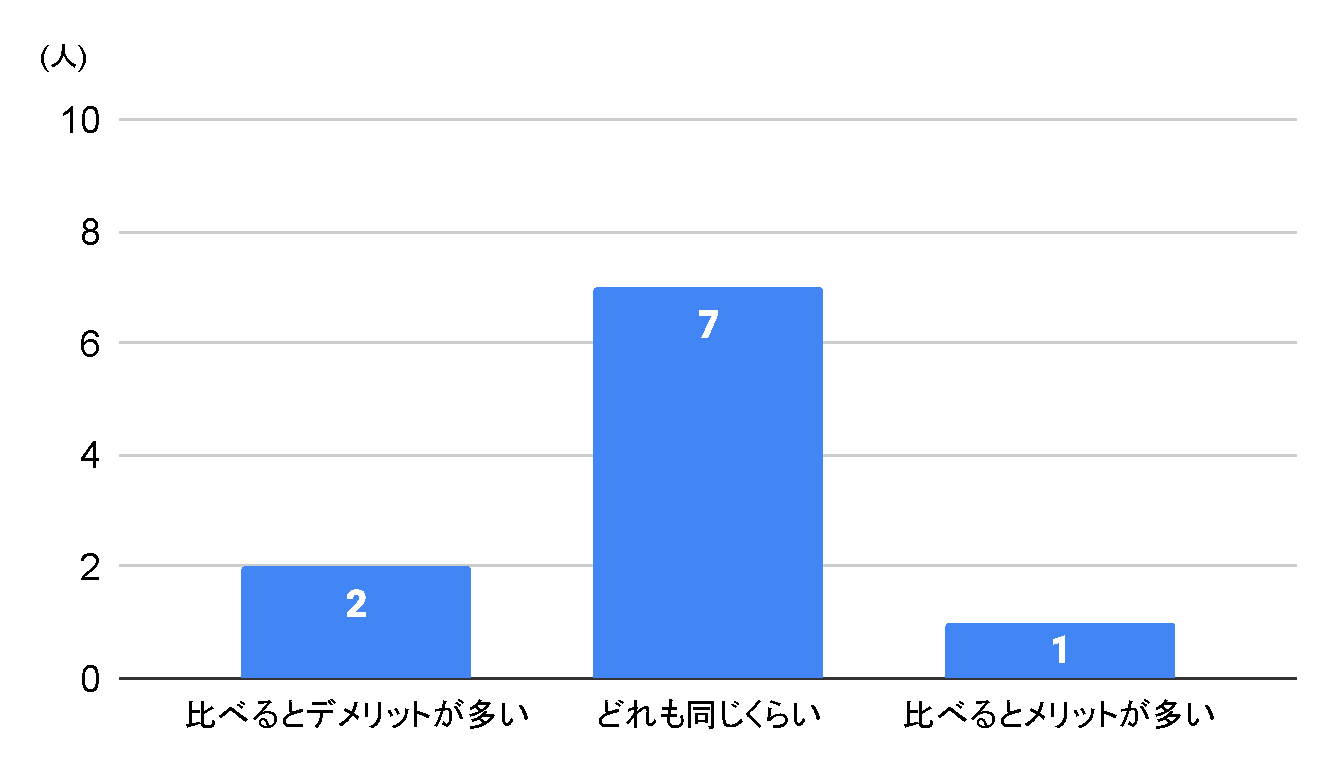
\includegraphics[keepaspectratio, scale=0.5]{PDF/比較後.pdf}
 \end{center}
 \caption{読書や映画鑑賞,スポーツ,友達と遊ぶことなど比べ,ゲームをプレイすることは利点があると思うか}
 \label{fig:比較後}
\end{figure}

最後にWebサイトの記事の内容に書かれたメリットが今後の子どもの発育や成長に影響があると思うかについては,図\ref{fig:記事影響}に示すように影響があると思うを選択した人が2人,やや良い影響があると思うを選択した人が4人,どちらとも言えないを選択した人が4人と少なからず影響があると考えた人が多かった.
またこの質問に対しての自由記述で以下のA,B,Cような意見が得られた.

\begin{itemize}
    \item[A.]  そんなメリットも確かにあるなと感じ、少なからず将来に影響はあると思った\\
    \item[B.]  学ぶことを意識してゲームをプレイできると思う。 \\
    \item[C.]  ゲームをする事により運動不足になると思う \\
\end{itemize}

\begin{figure}[H]
 \begin{center}
  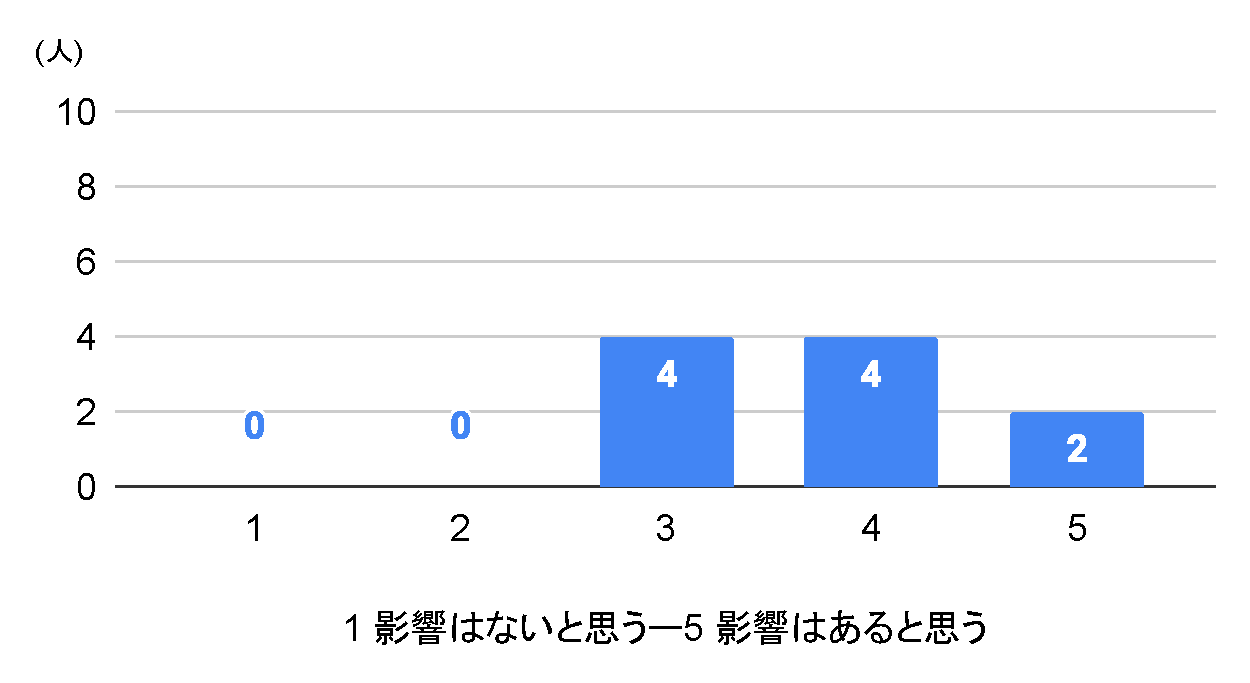
\includegraphics[keepaspectratio, scale=0.6]{PDF/記事影響.pdf}
 \end{center}
 \caption{記事に書かれたメリットは今後の子どもの発育・成長に影響があると思うか}
 \label{fig:記事影響}
\end{figure}

また「その他子どもへの影響についての意見」として以下のようなものが得られた.

\begin{itemize}
    \item[D.] ゲームによっては暴力表現があったりとデメリットのあるものもあるが,他の趣味と同じで親が見守り・指導すればよいことなので悪影響についてはゲームだけではないと思います
    \item[E.] 集中しすぎると画面に近づきすぎて,視力が悪くなるのが心配
    \item[F.] まだ子供が小さいので影響が少ないと思うが,大きくなるにつれて暴言が出ていたり,オンラインを使っていろんな人から得る影響が大きいと思う
\end{itemize}

\subsection{評価}
全体的なイメージの変化はWebサイトの記事によって悪いイメージから良いイメージへ改善された.
ゲームのパッケージやCM等にはプレイすることによる楽しさや面白さ,達成感などの娯楽的な魅力は大きく書かれているものの,教育的なメリットは書かれていなかった.
その点を本Webサイトで明示したことで今まで見えなかった利点を理解し良い影響もあるという考えに変化したのではないかと考えた.


勉強面では図\ref{fig:勉強前}と図\ref{fig:勉強後}のように悪い影響があると思うから良い影響があると思うに少し変化したが,表\ref{table:asmarqanque}の記述aにもあるように勉強できるゲームがあることは知っているものの,ゲームに夢中になることで学校や塾の宿題を疎かにしてしまうのではないかという懸念があり,考えの変化が少なかったのではないか.
また図\ref{fig:比較後}の読書等のメリットと比較したときメリットがあると答えた人が少ないように,読書などをした方がゲームをプレイするより学習できると考える人がいると考えられる.

友人関係やコミュニケーションについては現在マルチプレイや通話ツールを使いながらのゲームプレイは主流となっていて実際に子どもがそれらを使用し友人らとコミュニケーションを取っているとみられ,図\ref{fig:コミュ前}のように悪い影響があると思う人は少なかった.
Webサイトの記事にも多くのゲームでマルチプレイについて触れ,議論し考え協力しながらプレイできるなどと述べたため図\ref{fig:コミュ後}のように見た後の多少の変化があったと思われる.

感性についてはコミュニケーション面と同じようにゲームの紹介動画やCM等で創造力や表現力などが育てられるということは周知されていただろうと思われる.
Webサイトの記事では実際にゲームで土地変形や建物の建築が自由にでき個性を表現できることを具体的に示し,さらにマルチプレイで他の人の作品を鑑賞することもできるゲームがあるため,図\ref{fig:感性後}のように悪い影響があると考える人がなくなったのではないかと考えた.

知識や教養に関して図\ref{fig:知識前}と図\ref{fig:知識後}のように変化が少なかったのは多くのゲームは幅広い年齢層が対象で,小中学生にとっては大人や社会的に使用される表現や単語,物の名称等を自然に学べることを経験的に知っていたためではないか.
Webサイトの記事でもゲーム内で植物や動物の名称などの自然科学やローンや資金循環などの金融について学べることを示し,またストーリー内で英単語や外国の文化が学べることなどを記述した.

時間管理については勉強面でも挙げた表\ref{table:asmarqanque}の記述aのように学習や睡眠の時間を忘れ夢中になってしまう点があり親や子ども自身で管理しなくてはいけないためか,図\ref{fig:時間前}のように悪い影響があると思う人が多かった.
Webサイトの記事でもプレイ時間には中が必要であるとは記述したが,実際に管理することは難しいと考えているため図\ref{fig:時間後}のように変化が少なかったのではないか.

健康面では表\ref{table:asmarqanque}のgの意見や「その他子どもへの影響についての意見」のCと述べられているように運動をしなくなる点や,Fのように視力への懸念がある点によって図\ref{fig:健康前}のように悪い影響があると思う人が多く,図\ref{fig:健康後}のように見た後の回答も良い影響があると思う人が少なかったと考えられる.
Webサイトの記事で一部「リングフィットアドベンチャー」というゲームについて記述したため少し意見が好転したのではないか.

読書やスポーツ,映画鑑賞などの他の趣味や活動とメリットとの比較では,図\ref{fig:比較前}のWebサイトの記事を見る前のデメリットが多いと答えた人が見た後に図\ref{fig:比較後}のように2人に減りどれも同じくらいが増えたのは表\ref{アンケート調査}のi~ⅵの結果の通りで娯楽ゲームにも教育的なメリットがあると理解したと考える.
ただメリットが多いと答えた人が少なくどれも同じくらいと答える人が多かったのは,「その他子どもへの影響についての意見」のDのようにどのような活動でも親の見守りが必要だと考えがあるからだと考えられる.
またEの意見のようにどのようなゲームでも避けられない視力の問題やFの意見のようなマルチプレイによるコミュニケーション時の言葉遣いなどの問題があるため,完全にメリットがあるとは言えないのは事実である.

最後の質問で記事に書かれたメリットは今後子どもに影響があるかどうかでは,図\ref{fig:記事影響}に示すように6割の人が少なからず影響があると答えていて娯楽ゲームの教育的なメリットを明示し学習機会があることを理解してもらうという目的は達成できた結果となった.
ただどちらともいえないを選択した人が4人だったのは記述した教育的なメリットの根拠が薄いことやゲームの内容説明が足りない部分があること,ゲームのイメージがしにくい文章になっていた可能性がありこのような結果になったと考えられる.

また,時間管理や健康面については別に研究や調査が必要であることがわかった.
